% !TeX program = xelatex
\documentclass[14pt,a4paper]{extarticle}

% Compile in Overleaf with XeLaTeX.
\usepackage{fontspec}
\usepackage{polyglossia}
\setdefaultlanguage{russian}
\setotherlanguage{english}
\setmainfont{TeX Gyre Termes}
\setsansfont{TeX Gyre Heros}
\setmonofont{DejaVu Sans Mono}[Scale=0.82]

\usepackage{geometry}
\geometry{left=25mm,right=15mm,top=20mm,bottom=20mm}
\usepackage{graphicx}
\usepackage{adjustbox}
\usepackage{float}
\usepackage{xcolor}
\usepackage{hyperref}
\usepackage{fvextra}
\usepackage[most]{tcolorbox}
\usepackage{enumitem}
\usepackage{setspace}
\usepackage{titlesec}
\usepackage{caption}

\hypersetup{
    colorlinks=true,
    linkcolor=black,
    urlcolor=blue
}

\setstretch{1.15}
\setlength{\parindent}{1.25cm}
\setlength{\parskip}{0pt}
\titleformat{\section}{\normalfont\bfseries\large}{\thesection.}{0.5em}{}
\titleformat{\subsection}{\normalfont\bfseries}{\thesubsection.}{0.5em}{}

\newtcolorbox{codeframe}{
    colback=white,
    colframe=gray!70,
    boxrule=0.6pt,
    arc=4pt,
    left=2mm,
    right=2mm,
    top=2mm,
    bottom=2mm,
    breakable
}

\newenvironment{codeblock}{
    \begin{codeframe}
    \VerbatimEnvironment
    \begin{Verbatim}[fontsize=\scriptsize,breaklines=true,breakanywhere=true,tabsize=4]
}{
    \end{Verbatim}
    \end{codeframe}
}

% ====== Fill these fields before submission ======
\newcommand{\labvariant}{560711}
\newcommand{\studentone}{<ФИО первого студента>}
\newcommand{\studenttwo}{<ФИО второго студента>}
\newcommand{\groupname}{<Группа>}
\newcommand{\teacher}{<ФИО преподавателя>}

\begin{document}

\begin{titlepage}
    \centering
    Университет ИТМО\\
    Мегафакультет компьютерных технологий и управления\\
    Факультет программной инженерии и компьютерной техники\\[2.5cm]

    {\bfseries\Large ОТЧЕТ ПО ЛАБОРАТОРНОЙ РАБОТЕ №2\\[0.3cm]}
    {\bfseries\Large ОСНОВЫ ПРОГРАММНОЙ ИНЖЕНЕРИИ\\[0.8cm]}
    {\bfseries Вариант \labvariant\\[2.5cm]}

    \begin{flushright}
        Выполнили: \studentone,\\
        \studenttwo\\
        Группа: \groupname\\
        Проверил: \teacher
    \end{flushright}

    \vfill
    2026 год
\end{titlepage}

\section{Задание}

\begin{figure}[H]
    \centering
    \begin{adjustbox}{max width=\textwidth}
        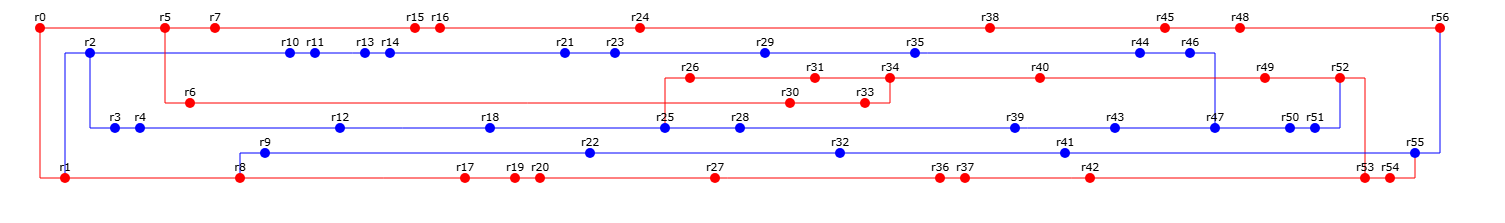
\includegraphics{block_scheme.png}
    \end{adjustbox}
    \caption{Блок-схема варианта \labvariant}
\end{figure}

Сконфигурировать в своём домашнем каталоге репозитории Mercurial и Git и загрузить в них начальную ревизию файлов с исходными кодами в соответствии с выданным вариантом.

Воспроизвести последовательность команд для систем контроля версий Mercurial и Git, осуществляющих операции над исходным кодом, приведённые на блок-схеме.

При составлении последовательности команд необходимо учитывать следующие условия:
\begin{itemize}[leftmargin=1.2cm]
    \item цвет элементов схемы указывает на пользователя, совершившего действие: красный --- первый, синий --- второй;
    \item цифры над узлами --- номер ревизии; ревизии создаются последовательно;
    \item необходимо разрешать конфликты между версиями, если они возникают.
\end{itemize}

\section{Реализация с использованием Git}

В Git-части лабораторной работы были созданы общий репозиторий \texttt{remote.git} и две рабочие копии: \texttt{user1\_work} для первого пользователя и \texttt{user2\_work} для второго пользователя. Первый пользователь настроен как \texttt{User Red}, второй пользователь --- как \texttt{User Blue}. Для соответствия номерам ревизий на схеме каждая ревизия помечалась тегом вида \texttt{r0}, \texttt{r1}, \ldots, \texttt{r56}.

Команды Git приведены ниже.

\begin{codeframe}
\VerbatimInput[fontsize=\scriptsize,breaklines=true,breakanywhere=true,tabsize=4]{commands_2.txt}
\end{codeframe}

\section{Реализация с использованием Mercurial}

\textbf{Поле для заполнения реализации Mercurial.} В этот раздел необходимо вставить команды второго участника, выполняющие аналогичное построение графа в Mercurial. Рекомендуется сохранить ту же структуру: настройки пользователей, функции для применения архива ревизии, функции для коммита, перехода между ветками, слияния, затем последовательность ревизий \texttt{r0--r56}.

\begin{codeblock}
# TODO: вставить реализацию Mercurial
#
# Пример структуры блока:
#
# red="User Red <red@example.com>"
# blue="User Blue <blue@example.com>"
#
# function Apply-ZipHg { ... }
# function Commit-HgRevision { ... }
# function Merge-HgRevision { ... }
#
# # r0
# # ...
#
# # r1-r56
# # ...
\end{codeblock}

\section{Вывод}

В ходе выполнения лабораторной работы были закреплены навыки работы с системами контроля версий Git и Mercurial. Для Git были настроены репозитории в домашнем каталоге пользователя, загружены исходные файлы из архивов ревизий и воспроизведена последовательность операций в соответствии с блок-схемой варианта. Были использованы операции создания веток, переключения между ветками, фиксации изменений, слияния веток и маркировки ревизий тегами. Практическая работа позволила лучше понять принципы построения графа истории, различия между ветками и ревизиями, а также роль merge-коммитов при объединении независимых линий разработки.

\end{document}
